\documentclass{beamer}
\usetheme[progressbar=frametitle]{metropolis}
% \setbeamertemplate{frame numbering}[fraction]
\useoutertheme{metropolis}
\useinnertheme{metropolis}
\usefonttheme{metropolis}
\usecolortheme{spruce}
\setbeamercolor{background canvas}{bg=white}
\usepackage[utf8]{inputenc}

% Code listings
\usepackage{listings}
\lstset{
  breaklines=true,
  keepspaces=true,
  basicstyle=\ttfamily
}
\lstset{columns=fullflexible,basicstyle=\ttfamily}
\usepackage{minted}
%\usemintedstyle{colorful}
\setminted{breaklines=true, baselinestretch=1}
%\DeclareBoolOption{newfloat}

% Graphics
\usepackage[labelsep=endash]{caption}
\usepackage{graphicx}
\usepackage{tikz}
\usetikzlibrary{
    automata,calc,trees,positioning,arrows,chains,shapes.geometric,
    decorations.pathreplacing,decorations.pathmorphing,shapes,
    matrix,shapes.symbols
}
\usepackage{newfloat}
\usepackage{subcaption}
\setlength{\abovecaptionskip}{10pt}
\setlength{\belowcaptionskip}{10pt}
\renewcommand{\thesubtable}{\roman{subtable}}
\renewcommand{\thesubfigure}{\roman{subfigure}}
\newenvironment{code}{\captionsetup{type=listing}}{}

%Information to be included in the title page:
\title[The Nuua Programming Language]{The Design of an Experimental Programming Language and its Translator}
\subtitle{The Nuua Programming Language}
\author{Èrik Campobadal Forés}
\institute{Universitat Politècnica de Catalunya}
\date{\today}


\begin{document}

\frame{\titlepage}
\begin{frame}<beamer>{Table of Contents}
    \begin{small}
    \tableofcontents[
        subsectionstyle=hide,
    ]
    \end{small}
\end{frame}
\section{Introduction}
\subsection{Objectives}
\begin{slide}
    \slidecaps{MAIN OBJECTIVES}
    \begin{itemize}
        \item Design an experimental programming language.
        \item Build a compiler and an interpreter for the language.
        \item Use a robust system architecture.
        \item Build a small standard library.
    \end{itemize}
\end{slide}

\subsection{System Architecture}
\begin{slide}
    \begin{figure}[H]
        \centering
        \includegraphics[height=0.85\textheight]{arch}
    \end{figure}
\end{slide}

\subsection{The Nuua Programming Language}
\begin{slide}
    \begin{block}{What is Nuua?}
        Nuua is a general-purpose high level programming language with an imperative paradigm and a statically typed system.
    \end{block}
    \vfill
    \begin{minted}{cpp}
fun main(argv: [string]) {
    print "Hello, World"
}
    \end{minted}
\end{slide}
\begin{slide}
    \begin{minted}{cpp}
class Triangle {
    b: float
    h: float
    fun area(): float -> (self.b * self.h) / 2.0
}

fun main(argv: [string]) {
    t := Triangle!{b: 10.0, h: 5.0}
    print "The area is: " + t.area() as string
}
    \end{minted}
\end{slide}
\begin{slide}
    \begin{minted}{cpp}
fun rec_fib(n: int): int {
    if n < 2 => return n
    return rec_fib(n - 2) + rec_fib(n - 1)
}

fun main(argv: [string]) {
    print rec_fib(25)
}
    \end{minted}
\end{slide}
\begin{slide}
    \begin{minted}[breaklines=false]{cpp}
use list_int_map from "list"

class Collection {
    numbers: [int]
    fun map(f: (int -> int)): Collection {
        list_int_map(self.numbers, f)
        return self
    }
}

fun multiply(n: int): int -> n * 2

fun main(argv: [string]) {
    c := Collection!{numbers: [1, 2, 3, 4, 5]}
    c.map(multiply).map(multiply)
    print c.numbers
}
    \end{minted}
\end{slide}

\subsection{Error Logging}
\begin{slide}
    \begin{figure}[H]
        \centering
        \includegraphics[height=0.6\textheight]{err}
        \caption{Example of error logging}
    \end{figure}
\end{slide}

\section{Lexical Analysis}
\subsection{Scanning the Source File}
\begin{slide}
    \begin{block}{Lexical Analysis}
        Transform a list of characters found in the source file into a list of
        tokens defined in the language.
    \end{block}
    \vfill
    \begin{figure}[H]
        \centering
        \begin{tikzpicture}
            [node distance=1cm]
            \node[block] (input) {List of characters};
            \node[block,right=of input] (lexer) {Lexer};
            \node[block,right=of lexer] (output) {List of tokens};
            \draw[line] (input) -- (lexer);
            \draw[line] (lexer) -- (output);
        \end{tikzpicture}
        \caption{Lexical analysis overview}
        \label{fig:lexer_overview}
    \end{figure}
\end{slide}
\begin{slide}
    \begin{figure}[H]
        \centering
        \includegraphics[width=0.9\textwidth]{finitestate}
        \caption{Example finite state machine for strings}
    \end{figure}
\end{slide}
\begin{slide}
    \begin{figure}[H]
        \centering
        \begin{tikzpicture}[node distance=1cm]
            % Nodes
            \node[square, minimum height=0.75cm, minimum width=1cm,] (n1) {...};
            \node[square, minimum height=0.75cm, minimum width=1cm, right of=n1] (n2) {\texttt{"}};
            \node[square, minimum height=0.75cm, minimum width=1cm, right of=n2] (n3) {\texttt{a}};
            \node[square, minimum height=0.75cm, minimum width=1cm, right of=n3] (n4) {\texttt{b}};
            \node[square, minimum height=0.75cm, minimum width=1cm, right of=n4] (n5) {\texttt{c}};
            \node[square, minimum height=0.75cm, minimum width=1cm, right of=n5] (n6) {\texttt{"}};
            \node[square, minimum height=0.75cm, minimum width=1cm, right of=n6] (n7) {...};
            % Lines
            \draw[line] ($(n2.south) + (0, -0.75)$) node[anchor=north] {\texttt{start\_ptr}} -- (n2);
            \draw[line] ($(n6.south) + (0, -0.75)$) node[anchor=north] {\texttt{current\_ptr}} -- (n6);
        \end{tikzpicture}
        \caption{Lexer scan technique}
        \label{fig:scanner}
    \end{figure}
    \begin{center}
        $\texttt{length} = \texttt{current\_ptr} - \texttt{start\_ptr} + 1$
    \end{center}
\end{slide}
\begin{slide}
    \begin{figure}[H]
        \centering
        \begin{tikzpicture}[node distance=1cm]
            % Nodes
            \node[square, minimum height=0.75cm, minimum width=1cm] (n1) {...};
            \node[square, minimum height=0.75cm, minimum width=1cm, right of=n1] (n2) {\texttt{w}};
            \node[square, minimum height=0.75cm, minimum width=1cm, right of=n2] (n3) {\texttt{h}};
            \node[square, minimum height=0.75cm, minimum width=1cm, right of=n3] (n4) {\texttt{i}};
            \node[square, minimum height=0.75cm, minimum width=1cm, right of=n4] (n5) {\texttt{l}};
            \node[square, minimum height=0.75cm, minimum width=1cm, right of=n5] (n6) {\texttt{e}};
            \node[square, minimum height=0.75cm, minimum width=1cm, right of=n6] (n7) {...};
            % Token nodes
            \node[square, anchor=west, minimum height=0.75cm] at ($(n1.south west) + (0, -2)$) (token) {\texttt{const char *start = \phantom{X}}};
            \node[square, minimum height=0.75cm, right = -0.025cm of token.east] (token1) {\texttt{const uint32\_t length = 5}};
            % Lines
            \draw[dot_arrow] ($(token.east) + (-0.2, -0.05)$) -- (n2.south);
        \end{tikzpicture}
        \caption{Token instance}
    \end{figure}
\end{slide}

\section{Syntactic Analysis}
\subsection{Technique}
\begin{slide}
    \begin{block}{Syntactic Analysis}
        Transform the list of tokens returned by the Lexer into an abstract syntax tree.
    \end{block}
    \vfill
    \begin{figure}[H]
        \centering
        \begin{tikzpicture}
            [node distance=1cm]
            \node[block] (input) {List of tokens};
            \node[block,right=of input] (parser) {Parser};
            \node[block,right=of lexer] (output) {Abstract syntax tree};
            \draw[line] (input) -- (parser);
            \draw[line] (parser) -- (output);
        \end{tikzpicture}
        \caption{Parser overview}
    \end{figure}
\end{slide}
\begin{slide}
    \slidecaps{MUST BE}
    \begin{itemize}
        \item Controlable (for error reporting).
        \item Easy to build.
        \item Fast enough.
        \item Handwritten (no generators).
    \end{itemize}
    \slidecaps{CANDIDATES}
    \begin{itemize}
        \item \textbf{Top-down recursive descend predictive parser.}
        \item Pratt parser (top-down operator-precedence parser).
    \end{itemize}
\end{slide}

\subsection{Abstract Syntax Tree}
\begin{slide}
    \begin{figure}[H]
        \centering
        \begin{subtable}{0.45\textwidth}
            \begin{minted}{cpp}
1 - 2 * -3
            \end{minted}
            \caption{Program}
        \end{subtable}
        \begin{subfigure}{0.45\textwidth}
            \centering
            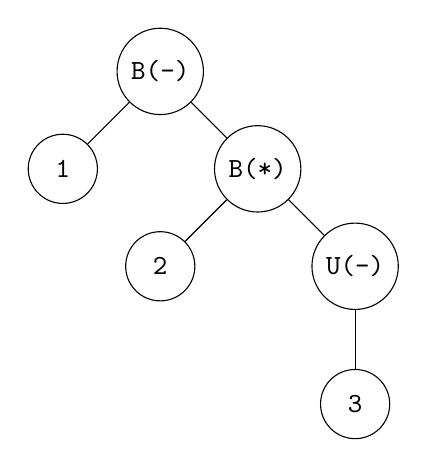
\begin{tikzpicture}[node distance=1.75cm]
                \node[state] (1) {\texttt{B(-)}};
                \node[state, below left of=1] (2) {\texttt{1}};
                \node[state, below right of=1] (3) {\texttt{B(*)}};
                \node[state, below left of=3] (4) {\texttt{2}};
                \node[state, below right of=3] (5) {\texttt{U(-)}};
                \node[state, below of=5] (6) {\texttt{3}};
                \draw (1) -- (2);
                \draw (1) -- (3);
                \draw (3) -- (4);
                \draw (3) -- (5);
                \draw (5) -- (6);
            \end{tikzpicture}
            \caption{Nuua AST}
        \end{subfigure}
        \caption{Example abstract syntax tree}
    \end{figure}
\end{slide}

\begin{slide}
    \begin{figure}[H]
        \centering
        \begin{subtable}{0.5\textwidth}
            \begin{minted}{cpp}
fun main(argv: [string]) {
    print 1 - 2 * -3
}
            \end{minted}
            \caption{Program}
        \end{subtable}
        \begin{subfigure}{0.45\textwidth}
            \centering
            \begin{minted}{cpp}
Function[main: <no-return>]
  Print
    Binary[-]
      Integer
      Binary[*]
        Integer
        Unary[-]
          Integer
            \end{minted}
            \caption{Nuua AST}
        \end{subfigure}
        \caption{Code example abstract syntax tree}
    \end{figure}
\end{slide}

\subsection{Path System}
\begin{slide}
    \slidecaps{PATH SYSTEM}
    \begin{itemize}
        \item Modules can be relative.
        \item Modules can be absolute.
        \item Modules can be on different paths.
    \end{itemize}
\end{slide}

\section{Semantic Analysis}
\subsection{Safety Checks}
\begin{slide}
    \begin{block}{Semantic Analysis}
        Append information to the AST and perform checks to ensure it's a valid program.
        If this checks succeed, the program is considered valid.
    \end{block}
    \vfill
    \slidecaps{IMPLEMENTED}
    \begin{itemize}
        \item Creation of the symbol table for each module and block scope.
        \item Expression type inference.
        \item Static type checking.
        \item Node information attachment.
    \end{itemize}
\end{slide}

\section{Code Generation}
\subsection{Instructions}
\begin{slide}
    \begin{block}{Code Generator}
        Transforms the AST into bytecode instructions ready to be executed by the virtual machine.
    \end{block}
    \vfill
    \begin{figure}[H]
        \centering
        \begin{tikzpicture}
            [node distance=1cm]
            \node[block] (input) {Abstract syntax tree};
            \node[block,right=of input] (codegen) {Code generator};
            \node[block,right=of lexer] (output) {List of opcodes};
            \draw[line] (input) -- (codegen);
            \draw[line] (codegen) -- (output);
        \end{tikzpicture}
        \caption{Code generator overview}
    \end{figure}
\end{slide}
\begin{slide}
    \slidecaps{IMPLEMENTED}
    \begin{itemize}
        \item Bytecode instructions similar to hardware instructions.
        \item 113 register-based instructions.
        \item Constant pool and globals creation.
        \item Frame sizes (registers needed).
        \item Optimizations
    \end{itemize}
\end{slide}

\subsection{Bytecode and Source File Relationship}
\begin{frame}[fragile]{Code Generator: Bytecode and Source File}
    \only<1>{
        {\footnotesize \textsc{PROBLEM}}
        \begin{itemize}
            \item Runtime exceptions require the source file information.
            \item Requires the file name, the line and the column.
            \item Each opcode require this information because it can fail.
            \item Very memory inefficient.
        \end{itemize}
        {\footnotesize \textsc{SOLUTION}}
        \begin{itemize}
            \item Register only the changes on the file, line or column.
            \item Guess the file, line and column based on the current opcode.
        \end{itemize}
    }
    \begin{onlyenv}<2>
        \begin{figure}[H]
	        \centering
            \begin{subtable}{0.3\textwidth}
                \begin{minted}[linenos]{cpp}
a: int = 10
b: int = a - 10
print a / b
                \end{minted}
		    \caption{Input program}
	        \end{subtable}
	        \begin{subtable}{0.6\textwidth}
                \begin{minted}{cpp}
LOAD_C  R-00000 C-00000
LOAD_C  R-00002 C-00001
SUB_INT R-00001 R-00000 R-00002
DIV_INT R-00001 R-00000 R-00001
PRINT   R-00001
                \end{minted}
            \caption{Bytecode generated}
	        \end{subtable}
            \begin{subtable}{0.3\textwidth}
                {\footnotesize \textsc{CONDITION}}\\
                Highest index that is lower or equal to the crash index.
	        \end{subtable}
            \begin{subtable}{0.6\textwidth}
                \centering
                \begin{tabular}{ l l }
                    \textbf{Opcode Index} & \textbf{Line number} \\
                    0 & 1 \\
                    3 & 2 \\
                    10 & 3 \\
                \end{tabular}
            \caption{Registered line changes}
	        \end{subtable}
        \caption{Runtime exception}
        \end{figure}
    \end{onlyenv}
\end{frame}

\section{Optimizations}
\subsection{Constant Folding}
\begin{frame}[fragile]{Code Generator Optimizations: Basic Constant Folding}
    \only<1>{
        {\footnotesize \textsc{IMPLEMENTED}}
        \begin{itemize}
            \item Very basic constant folding on lists and dictionaries.
        \end{itemize}
        {\footnotesize \textsc{IMPROVEMENT}}
        \begin{itemize}
            \item Reduce the number of opcodes.
            \item Improve runtime performance.
        \end{itemize}
    }
    \begin{onlyenv}<2>
        \begin{figure}[H]
	        \centering
            \begin{subtable}{0.3\textwidth}
                \begin{minted}[linenos]{cpp}
print [1, 2, 3]
a: int = 3
print [1, 2, a]
                \end{minted}
		    \caption{Input program}
	        \end{subtable}
	        \begin{subtable}{0.6\textwidth}
                \begin{minted}{cpp}
PRINT_C C-00000
LOAD_C  R-00000 C-00001
LOAD_C  R-00001 C-00002
LPUSH_C R-00001 C-00003
LPUSH_C R-00001 C-00004
LPUSH   R-00001 R-00000
PRINT   R-00001
                \end{minted}
            \caption{Optimized bytecode generated}
	        \end{subtable}
        \caption{List constant folding}
        \end{figure}
    \end{onlyenv}
\end{frame}

\subsection{Register allocation}
\begin{slide}
    \slidecaps{PROBLEM}
    \begin{itemize}
        \item How long is the value of a register needed?
        \item Can we re-use the registers?
    \end{itemize}
    \slidecaps{IMPLEMENTED}
    \begin{itemize}
        \item Linear scan register allocation.
    \end{itemize}
    \slidecaps{IMPROVEMENT}
    \begin{itemize}
        \item Significant memory reduction.
    \end{itemize}
\end{slide}
\begin{slide}
    \begin{figure}[H]
        \centering
        \begin{subtable}{0.3\textwidth}
            \begin{minted}[linenos]{cpp}
a: int = 10
b: int = 20
print a + b
c: int = a
print c
            \end{minted}
        \caption{Input program}
        \end{subtable}
        \begin{subtable}{0.6\textwidth}
            \begin{tikzpicture}
                \draw[thick, ->] (0,0) -- (5,0) node[anchor=north] {\emph{Line}};
                \draw[thick] (0,0) -- (0,4) node[anchor=east] {\emph{Variable}};
                \node[anchor=east] at (0, 3) {a};
                \node[anchor=east] at (0, 2) {b};
                \node[anchor=east] at (0, 1) {c};
                \draw[dashed, *-*] (-0.075, 3) -- (3.075, 3);
                \draw[dashed, *-*] (0.925, 2) -- (2.075, 2);
                \draw[dashed, *-*] (2.925, 1) -- (4.075, 1);
                \node[anchor=north] at (4, 0) {5};
                \node[anchor=north] at (3, 0) {4};
                \node[anchor=north] at (2, 0) {3};
                \node[anchor=north] at (1, 0) {2};
                \node[anchor=north] at (0, 0) {1};
            \end{tikzpicture}
        \caption{Variable lifetime}
        \end{subtable}
    \caption{Variable lifetime of a program}
    \end{figure}
\end{slide}
\begin{slide}
    \begin{figure}[H]
        \centering
        \begin{subtable}{0.3\textwidth}
            \begin{minted}[linenos]{cpp}
a: int = 10
b: int = 20
print a + b
c: int = a
print c
            \end{minted}
        \caption{Input program}
        \end{subtable}
        \begin{subtable}{0.6\textwidth}
            \begin{minted}{cpp}
LOAD_C  R-00000 C-00000
LOAD_C  R-00001 C-00001
ADD_INT R-00001 R-00000 R-00001
PRINT   R-00001
MOVE    R-00001 R-00000
PRINT   R-00001
            \end{minted}
        \caption{Optimized bytecode generated}
        \end{subtable}
    \caption{Register allocation optimization of a program}
    \end{figure}
\end{slide}

\section{Virtual Machine}
\subsection{Value Stack and Call stack}
\begin{slide}
    \begin{block}{Virtual Machine}
        Execute the bytecode instructions generated.
    \end{block}
    \vfill
    \slidecaps{IMPLEMENTED}
    \begin{itemize}
        \item A call stack.
        \item A value stack to pass parameters.
        \item Automatic call to the \texttt{main} function with \texttt{argv} argument.
    \end{itemize}
\end{slide}
\begin{slide}
    \begin{figure}[H]
        \centering
        \begin{subtable}{0.5\textwidth}
            \begin{minted}{cpp}
fun mul(a: int): int {
    return a * 2
}

fun main(argv: [string]) {
    print mul(10)
}
            \end{minted}
        \caption{Input program}
        \end{subtable}
        \begin{subtable}{0.45\textwidth}
            \only<1>{
                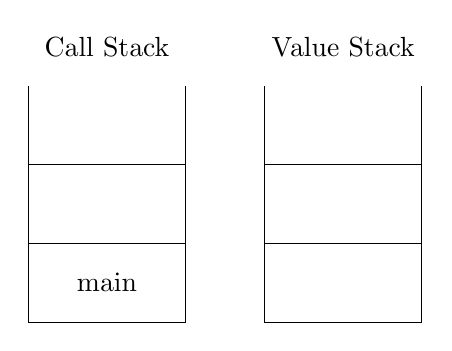
\begin{tikzpicture}
                    % Labels
                    \node at (1, 3.5) {Call Stack};
                    \node at (4, 3.5) {Value Stack};
                    % Stack
                    \draw[] (0, 0) -- (2, 0);
                    \draw[] (0, 1) -- (2, 1);
                    \draw[] (0, 2) -- (2, 2);
                    \draw[] (0, 0) -- (0, 3);
                    \draw[] (2, 0) -- (2, 3);
                    % Elements
                    \node at (1, 0.5) {main};
                    % Stack
                    \draw[] (3, 0) -- (5, 0);
                    \draw[] (3, 1) -- (5, 1);
                    \draw[] (3, 2) -- (5, 2);
                    \draw[] (3, 0) -- (3, 3);
                    \draw[] (5, 0) -- (5, 3);
                    % Elements
                \end{tikzpicture}
            }
            \only<2>{
                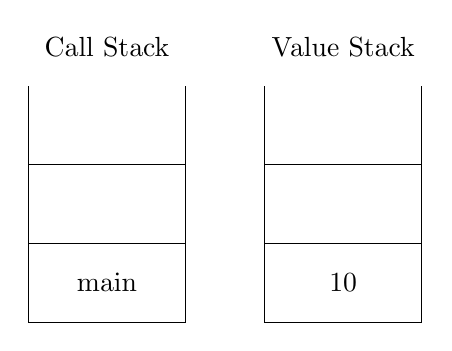
\begin{tikzpicture}
                    % Labels
                    \node at (1, 3.5) {Call Stack};
                    \node at (4, 3.5) {Value Stack};
                    % Stack
                    \draw[] (0, 0) -- (2, 0);
                    \draw[] (0, 1) -- (2, 1);
                    \draw[] (0, 2) -- (2, 2);
                    \draw[] (0, 0) -- (0, 3);
                    \draw[] (2, 0) -- (2, 3);
                    % Elements
                    \node at (1, 0.5) {main};
                    % \node at (1, 1.5) {mul};
                    % Stack
                    \draw[] (3, 0) -- (5, 0);
                    \draw[] (3, 1) -- (5, 1);
                    \draw[] (3, 2) -- (5, 2);
                    \draw[] (3, 0) -- (3, 3);
                    \draw[] (5, 0) -- (5, 3);
                    % Elements
                    \node at (4, 0.5) {10};
                \end{tikzpicture}
            }
            \only<3>{
                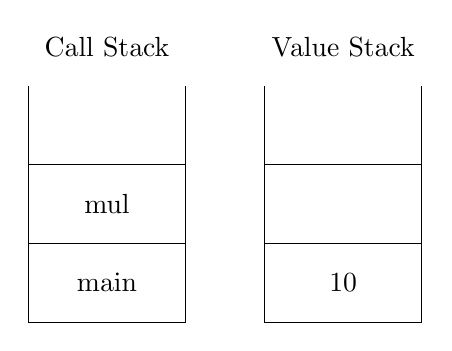
\begin{tikzpicture}
                    % Labels
                    \node at (1, 3.5) {Call Stack};
                    \node at (4, 3.5) {Value Stack};
                    % Stack
                    \draw[] (0, 0) -- (2, 0);
                    \draw[] (0, 1) -- (2, 1);
                    \draw[] (0, 2) -- (2, 2);
                    \draw[] (0, 0) -- (0, 3);
                    \draw[] (2, 0) -- (2, 3);
                    % Elements
                    \node at (1, 0.5) {main};
                    \node at (1, 1.5) {mul};
                    % Stack
                    \draw[] (3, 0) -- (5, 0);
                    \draw[] (3, 1) -- (5, 1);
                    \draw[] (3, 2) -- (5, 2);
                    \draw[] (3, 0) -- (3, 3);
                    \draw[] (5, 0) -- (5, 3);
                    % Elements
                    \node at (4, 0.5) {10};
                \end{tikzpicture}
            }
            \only<4>{
                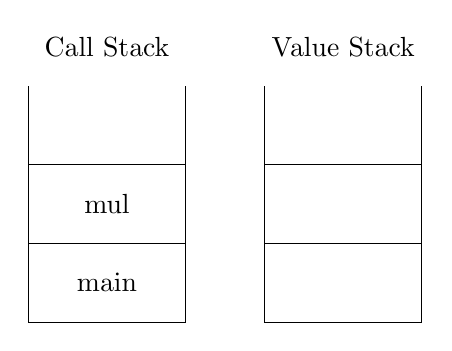
\begin{tikzpicture}
                    % Labels
                    \node at (1, 3.5) {Call Stack};
                    \node at (4, 3.5) {Value Stack};
                    % Stack
                    \draw[] (0, 0) -- (2, 0);
                    \draw[] (0, 1) -- (2, 1);
                    \draw[] (0, 2) -- (2, 2);
                    \draw[] (0, 0) -- (0, 3);
                    \draw[] (2, 0) -- (2, 3);
                    % Elements
                    \node at (1, 0.5) {main};
                    \node at (1, 1.5) {mul};
                    % Stack
                    \draw[] (3, 0) -- (5, 0);
                    \draw[] (3, 1) -- (5, 1);
                    \draw[] (3, 2) -- (5, 2);
                    \draw[] (3, 0) -- (3, 3);
                    \draw[] (5, 0) -- (5, 3);
                    % Elements
                    % \node at (4, 0.5) {10};
                \end{tikzpicture}
            }
            \only<5>{
                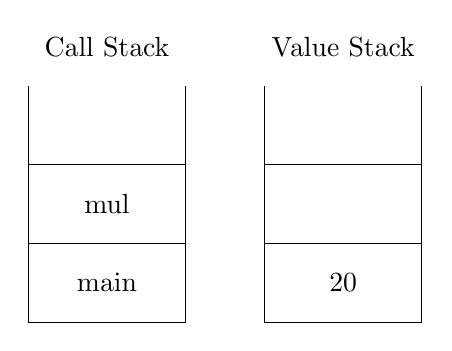
\begin{tikzpicture}
                    % Labels
                    \node at (1, 3.5) {Call Stack};
                    \node at (4, 3.5) {Value Stack};
                    % Stack
                    \draw[] (0, 0) -- (2, 0);
                    \draw[] (0, 1) -- (2, 1);
                    \draw[] (0, 2) -- (2, 2);
                    \draw[] (0, 0) -- (0, 3);
                    \draw[] (2, 0) -- (2, 3);
                    % Elements
                    \node at (1, 0.5) {main};
                    \node at (1, 1.5) {mul};
                    % Stack
                    \draw[] (3, 0) -- (5, 0);
                    \draw[] (3, 1) -- (5, 1);
                    \draw[] (3, 2) -- (5, 2);
                    \draw[] (3, 0) -- (3, 3);
                    \draw[] (5, 0) -- (5, 3);
                    % Elements
                    \node at (4, 0.5) {20};
                \end{tikzpicture}
            }
            \only<6>{
                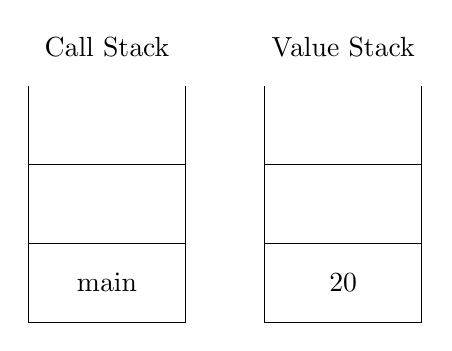
\begin{tikzpicture}
                    % Labels
                    \node at (1, 3.5) {Call Stack};
                    \node at (4, 3.5) {Value Stack};
                    % Stack
                    \draw[] (0, 0) -- (2, 0);
                    \draw[] (0, 1) -- (2, 1);
                    \draw[] (0, 2) -- (2, 2);
                    \draw[] (0, 0) -- (0, 3);
                    \draw[] (2, 0) -- (2, 3);
                    % Elements
                    \node at (1, 0.5) {main};
                    % Stack
                    \draw[] (3, 0) -- (5, 0);
                    \draw[] (3, 1) -- (5, 1);
                    \draw[] (3, 2) -- (5, 2);
                    \draw[] (3, 0) -- (3, 3);
                    \draw[] (5, 0) -- (5, 3);
                    % Elements
                    \node at (4, 0.5) {20};
                \end{tikzpicture}
            }
            \only<7>{
                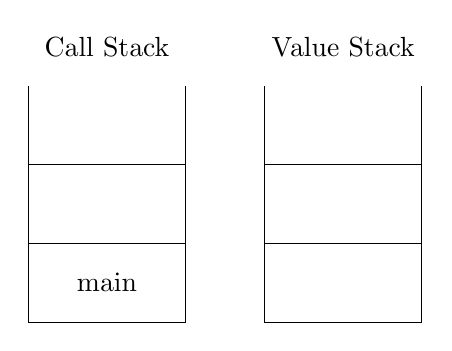
\begin{tikzpicture}
                    % Labels
                    \node at (1, 3.5) {Call Stack};
                    \node at (4, 3.5) {Value Stack};
                    % Stack
                    \draw[] (0, 0) -- (2, 0);
                    \draw[] (0, 1) -- (2, 1);
                    \draw[] (0, 2) -- (2, 2);
                    \draw[] (0, 0) -- (0, 3);
                    \draw[] (2, 0) -- (2, 3);
                    % Elements
                    \node at (1, 0.5) {main};
                    % Stack
                    \draw[] (3, 0) -- (5, 0);
                    \draw[] (3, 1) -- (5, 1);
                    \draw[] (3, 2) -- (5, 2);
                    \draw[] (3, 0) -- (3, 3);
                    \draw[] (5, 0) -- (5, 3);
                    % Elements
                \end{tikzpicture}
            }
        \caption{Stacks}
        \end{subtable}
    \caption{Stack usage on program execution}
    \end{figure}
\end{slide}

\subsection{Instruction Dispatch}
\begin{frame}[fragile]{Virtual Machine: Instruction Dispatch}
    \only<1>{
        {\footnotesize \textsc{PROBLEM}}
        \begin{itemize}
            \item Threaded dispatch is not ANSI C compilant.
        \end{itemize}
        {\footnotesize \textsc{SOLUTION}}
        \begin{itemize}
            \item Use a switch dispatch
        \end{itemize}
        {\footnotesize \textsc{TRADEOFF}}
        \begin{itemize}
            \item ANSI C compilant.
            \item Less efficient than a threaded dispatch.
            \item Simple to implement.
        \end{itemize}
    }
\end{frame}

\section{Application}
\subsection{Job}
\begin{slide}
    \begin{block}{Application}
        Setup the application and fire up the virtual machine.
    \end{block}
    \vfill
    \slidecaps{IMPLEMENTED}
    \begin{itemize}
        \item Command line argument parsing.
        \item Extension to multiple application types (Prompt, stdin, File, etc.).
        \item Creation of the initial \texttt{argv: [string]} argument for the \texttt{main} function.
    \end{itemize}
\end{slide}

\section{Conclusions}
\subsection{General Objectives}
\begin{slide}
    \slidecaps{IN GENERAL}
    \begin{itemize}
        \item Primary objectives completed.
        \item Competitive and performant interpreter.
        \item Benchmarking is hard.
    \end{itemize}
    \slidecaps{FURTHER EVOLUTION}
    \begin{itemize}
        \item C foreign function interface (FFI).
        \item Propper I/O interface.
        \item Function overloading and generics.
        \item Extended standard library.
        \item Website (\url{https://nuua.io}) and package manager.
    \end{itemize}
\end{slide}

\subsection{Curiosities}
\begin{slide}
    \begin{itemize}
        \item $5k$ \texttt{C++} lines.
        \item $2.3k$ \texttt{C++} header lines.
        \item $1.4k$ Comment lines.
        \item $7.5k$ Total project lines.
        \item $500KB$ Total release binary size (Windows).
        \item Nuua is available for Linux and Windows under the MIT license at \url{http://nuua.io/latest}
    \end{itemize}
\end{slide}


\end{document}
